\documentclass[10pt]{beamer}
\usepackage{bm}
\usetheme[progressbar=frametitle]{metropolis}
\usepackage{appendixnumberbeamer}
\usepackage{listings}
\usepackage{xcolor}

\definecolor{codegreen}{rgb}{0,0.6,0}
\definecolor{codegray}{rgb}{0.5,0.5,0.5}
\definecolor{codepurple}{rgb}{0.58,0,0.82}
\definecolor{backcolour}{rgb}{0.98,0.98,0.98}
\usepackage{animate}
\usepackage{media9}

\lstdefinestyle{mystyle}{
    backgroundcolor=\color{backcolour},
    commentstyle=\color{codegreen},
    keywordstyle=\color{magenta},
    numberstyle=\tiny\color{codegray},
    stringstyle=\color{codepurple},
    basicstyle=\ttfamily\scriptsize,
    breakatwhitespace=false,
    breaklines=true,
    captionpos=b,
    keepspaces=true,
    numbers=left,
    numbersep=5pt,
    showspaces=false,
    showstringspaces=false,
    showtabs=false,
    tabsize=2,
    frame=tb
}
\lstset{style=mystyle}

\usepackage{booktabs}
\usepackage[scale=2]{ccicons}
\usepackage{pgfplots}
\pgfplotsset{compat=1.18}
\usepackage{xspace}
\usepackage{amsmath}
\usepackage{amssymb}
\usepackage{graphicx}
\newcommand{\vect}[1]{\bm{#1}}
\newcommand{\op}[1]{\mathcal{#1}}
\usepackage[style=numeric]{biblatex}
\addbibresource{ref.bib}
\providecommand{\argmin}{\operatorname*{argmin}}

\title{Generative Denoising for Medical Image Reconstruction}
\subtitle{Using Score-Based Diffusion Models}
\date{}
\author{Siddhant Chaurasia}

\begin{document}

\maketitle

\begin{frame}{Table of contents}
  \setbeamertemplate{section in toc}[sections numbered]
  \tableofcontents
\end{frame}

\section{Motivation \& Background}

\begin{frame}{Clinical Challenge in CT Imaging}
  \begin{columns}[T]
    \begin{column}{0.6\textwidth}
      \textbf{Key challenges in CT imaging:}
      \begin{itemize}
        \item Radiation dose concerns; trade-off between image quality and radiation exposure
        \item Need for fast acquisition to reduce motion artifacts
      \end{itemize}

      \bigskip
      \textbf{Sparse-view CT as a solution:}
      \begin{itemize}
        \item Reduces radiation dose
        \item Faster acquisition times
        \item But creates undersampled data → reconstruction problem
      \end{itemize}
    \end{column}

    \begin{column}{0.4\textwidth}
        \begin{figure}
            \centering
            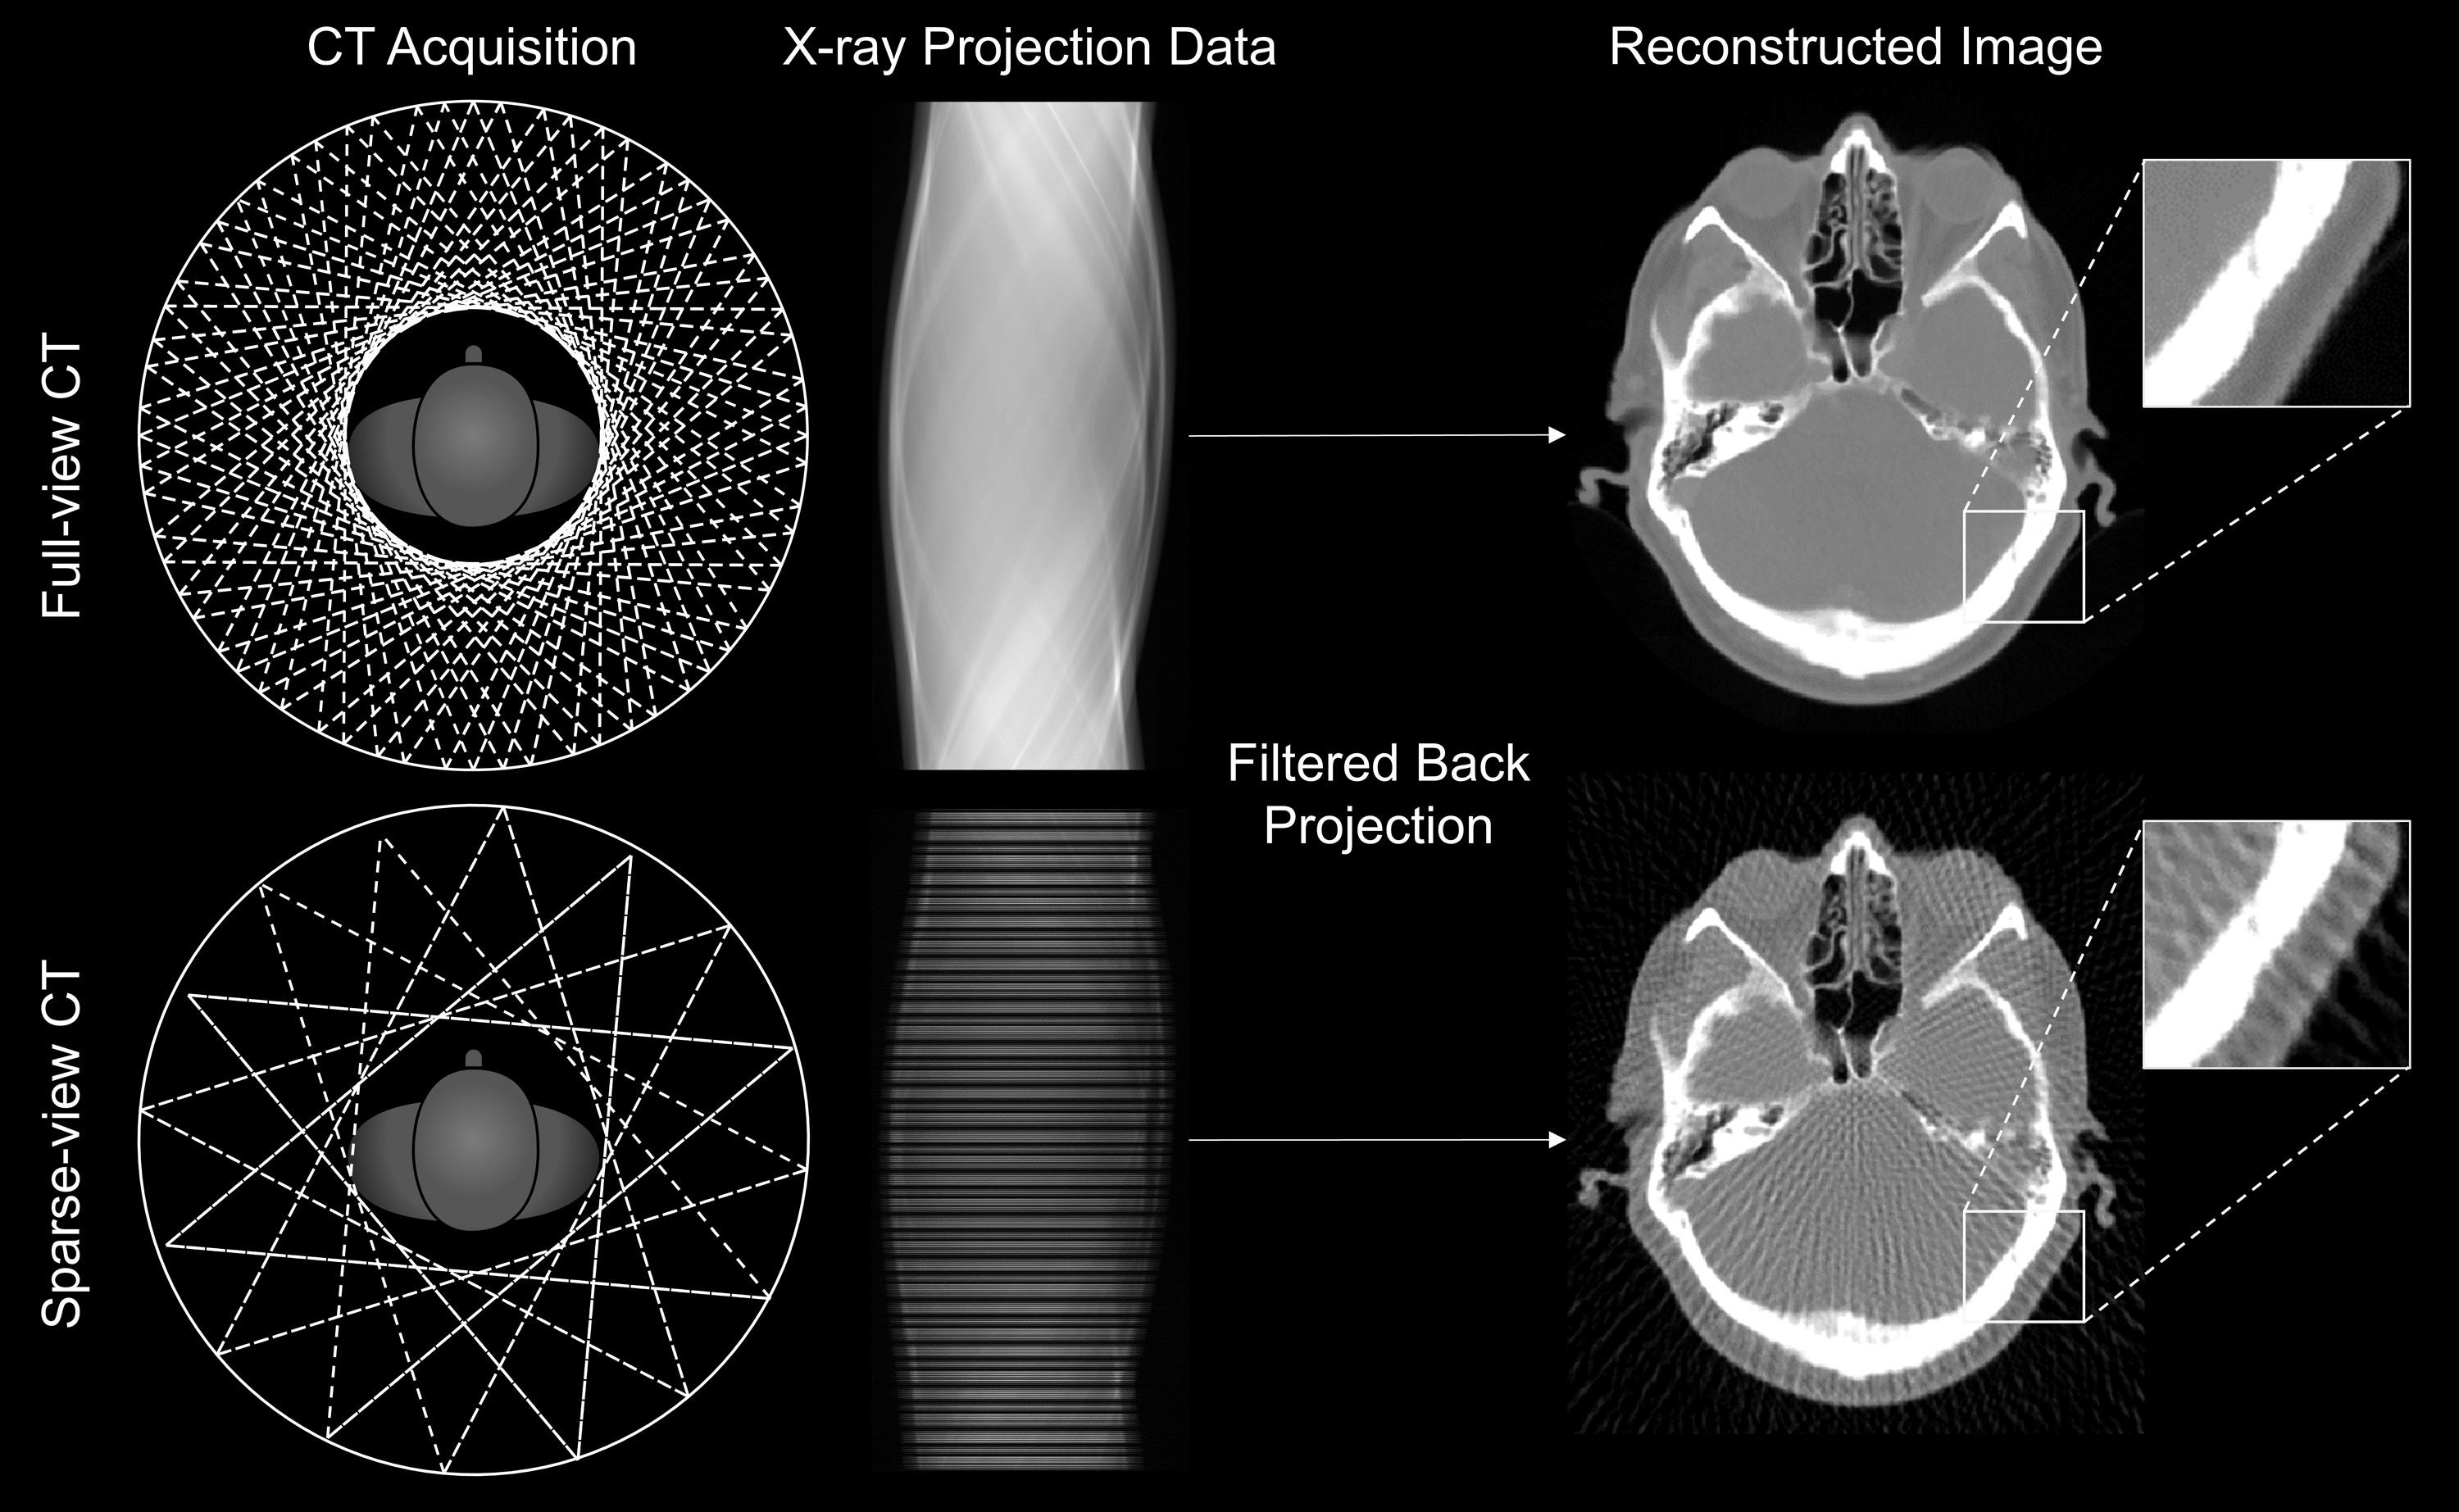
\includegraphics[width=1.1\textwidth]{ct.jpg}
            \caption{Sparse views CT (Adapted from Chung2022\cite{Chung2022}).}
        \end{figure}


      \begin{alertblock}{Research Goal}
        Develop advanced reconstruction algorithms to produce high-quality images from limited data
      \end{alertblock}
    \end{column}
  \end{columns}
\end{frame}

\begin{frame}{CT Reconstruction}

  \textbf{Forward Model:}
  \begin{align*}
    \vect{y} = \op{A}\vect{x} + \vect{\eta}
  \end{align*}
  \footnotesize
  \textbf{Where:} \\
  $\vect{y}$: Measured scanner data (sinogram). \\
  $\op{A}$: System model (Radon transform, describes scanner physics). \\
  $\vect{x}$: The true underlying image we want to find. \\
  $\vect{\eta}$: Measurement noise and model inaccuracies.
  \normalsize

  \bigskip

  \textbf{Inverse Problem:}
  \begin{align*}
       \hat{\vect{x}} = \operatorname*{argmin}_{\vect{x}} \underbrace{\|\op{A}\vect{x} - \vect{y}\|^2}_{\substack{\text{Data Fidelity}\\\text{(Match measurements)}}} + \underbrace{\lambda R(\vect{x})}_{\substack{\text{Regularization}\\\text{(Incorporate prior knowledge)}}}
  \end{align*}
  \footnotesize
  \textbf{Goal:} Find the image estimate $\hat{\vect{x}}$ that best fits the measurements while also incorporating prior knowledge or assumptions about the image via the regularizer $R(\vect{x})$. The parameter $\lambda$ controls the trade-off.
  \normalsize

\end{frame}

\section{Diffusion Models}

\begin{frame}{Diffusion Models: Core Idea}
  \textbf{Generate data by learning to reverse a noise-adding process.}

  \medskip
  \textbf{How it Works:}
  \begin{itemize}
    \item \textbf{Forward:} Add noise gradually. (Fixed)
    \item \textbf{Reverse:} Learn to remove noise step by step. (Generative)
  \end{itemize}
    \begin{figure}
            \centering
            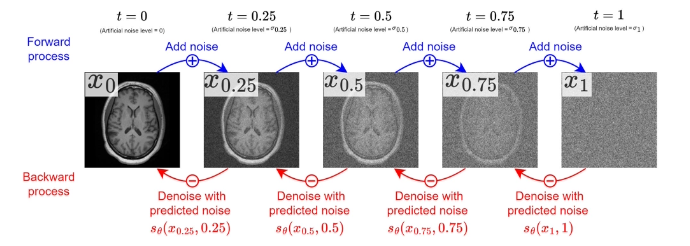
\includegraphics[width=\textwidth]{diff_mod.png}
            \caption{Diffusion Process (Adapted from Reader24) \cite{95846d1d06ff4241b5527fe62da68126}.}
        \end{figure}
\end{frame}

\section{Task \& Dataset}

\begin{frame}{Generative Denoising of CT Patches}
  \textbf{Objective:} Reconstruct clean 28x28 CT image patches ($\vect{x}$) from noisy versions ($\vect{y}$), where noise is simulated as additive white Gaussian noise ($\vect{y} = \vect{x} + \mathcal{N}(0, \sigma_n^2 \mathbf{I})$).

  \medskip
  \textbf{Challenge:} Effectively remove significant noise ($\sigma_n = 0.3$ in [-1, 1] space) while preserving fine anatomical details within small image patches.

  \medskip
  \textbf{My Approach} Utilize a \alert{Score-Based Diffusion Model}, conditioned on the noisy input image $\vect{y}$, to perform generative denoising via a learned reverse process.

\end{frame}

\begin{frame}{Dataset: OrganAMNIST (from MedMNIST)}
  \begin{columns}[T,onlytextwidth]
    \column{0.45\textwidth}
      \begin{itemize}\setlength\itemsep{0.8em}
        \item Publicly available MedMNIST~\cite{yang2023medmnist}
        \item Derived from the Liver Tumor Segmentation Benchmark (LiTS) CT scans.
        \item Content: 2D axial CT patches ($28\times28$ grayscale) centered on 11 organs (labels discarded).
        \item Preprocessing: HU values windowed using an abdominal window; images normalized to $[-1,1]$.
      \end{itemize}

    \column{0.55\textwidth}
      \centering
      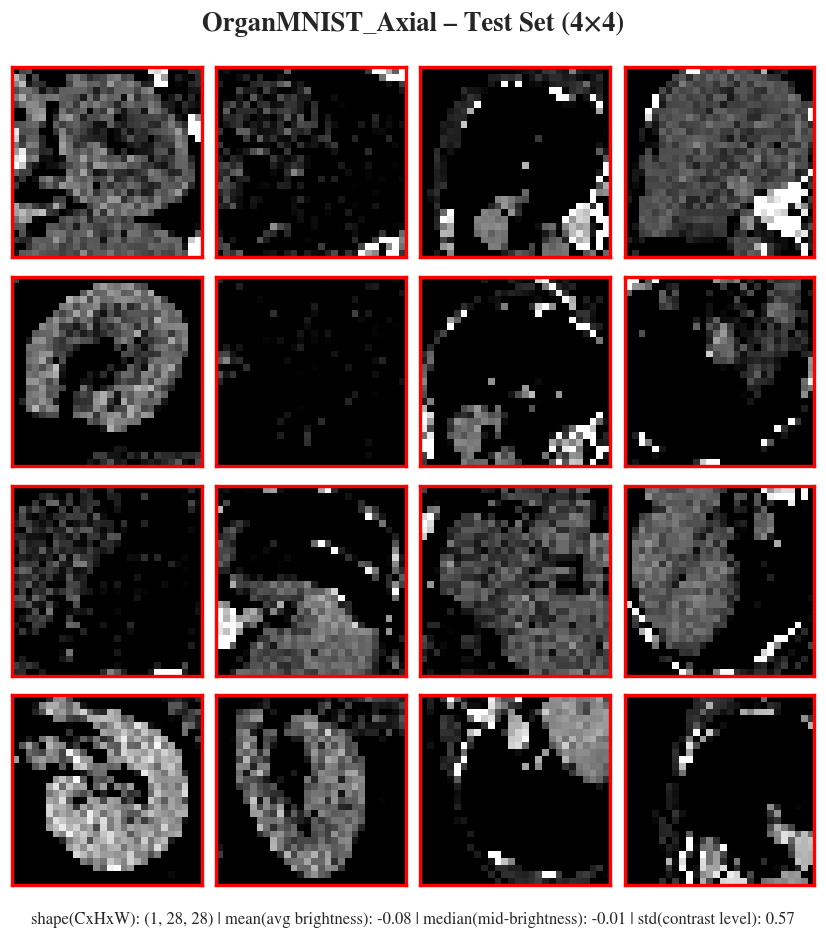
\includegraphics[width=\linewidth,height=0.46\textheight,keepaspectratio]{test.png}\\[1ex]
      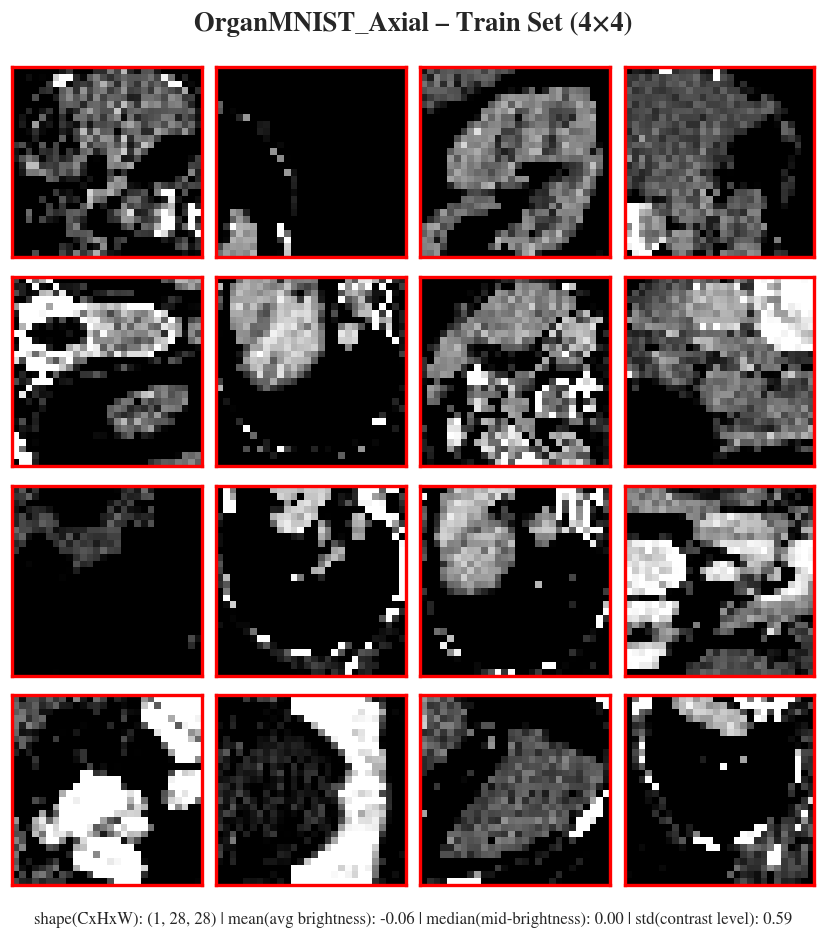
\includegraphics[width=\linewidth,height=0.46\textheight,keepaspectratio]{train.png}
  \end{columns}
\end{frame}

\section{Stochastic Differential Equations in Diffusion Models}
\begin{frame}{VP-SDE: Mathematical Formulation}
  \begin{columns}[T]
    \begin{column}{0.65\textwidth}
      \textbf{Forward Process (Data $\rightarrow$ Noise)}
      \begin{itemize} \itemsep -0.1cm
        \item Continuous SDE ($t \in [0, 1]$):
          \vspace{-0.1cm}
          \begin{equation*}
            d\mathbf{x} = -\frac{1}{2}\beta(t)\mathbf{x}dt + \sqrt{\beta(t)}d\mathbf{w}
          \end{equation*}
          \vspace{-0.3cm}
        \item Gaussian Marginal:
          \begin{equation*}
            p(\mathbf{x}_t|\mathbf{x}_0) = \mathcal{N}(\mathbf{x}_t; \sqrt{\bar{\alpha}_t}\mathbf{x}_0, (1-\bar{\alpha}_t)\mathbf{I})
          \end{equation*}
          \vspace{-0.3cm}
        \item Direct Sampling Formula:
          \begin{equation*}
            \mathbf{x}_t = \sqrt{\bar{\alpha}_t}\mathbf{x}_0 + \sqrt{1-\bar{\alpha}_t}\mathbf{z}
          \end{equation*}
      \end{itemize}
    \end{column}

    \begin{column}{0.35\textwidth}
      \textbf{Key Terms:}
      \begin{itemize} \itemsep -0.1cm
        \item $\beta(t)$: Noise schedule
        \item $\bar{\alpha}_t$: Cumulative product\\ $\prod_{i=1}^{t}(1-\beta_i)$
        \item $\mathbf{w}$: Wiener process
        \item $\mathbf{z} \sim \mathcal{N}(\mathbf{0}, \mathbf{I})$
      \end{itemize}

      \begin{alertblock}{Key Insight}
        VP-SDE gradually transforms data into noise with controlled variance, enabling flexible sampling.
      \end{alertblock}
    \end{column}
  \end{columns}
\end{frame}

\begin{frame}[fragile]{VP-SDE: Implementation}
  \begin{columns}[T]
    \begin{column}{0.6\textwidth}
      \textbf{Cosine Noise Schedule:}
      \begin{lstlisting}[language=Python,
                            basicstyle=\ttfamily\tiny,
                            numbers=none,
                            frame=single]
s = 0.008
steps = torch.linspace(0, n_steps, n_steps + 1)

f_t = torch.cos(((steps / n_steps) + s) /
       (1 + s) * math.pi / 2) ** 2
alpha_bar = f_t / f_t[0]

betas = (1 - (alpha_bar[1:] / alpha_bar[:-1]))
       .clamp(0.0001, 0.9999)

sqrt_alpha_bar = torch.sqrt(alpha_bar[1:])
sqrt_one_minus_alpha_bar = torch.sqrt(
    1 - alpha_bar[1:])
      \end{lstlisting}
    \end{column}

    \begin{column}{0.4\textwidth}
      \vspace{0.5cm}
      \begin{figure}
          \centering
          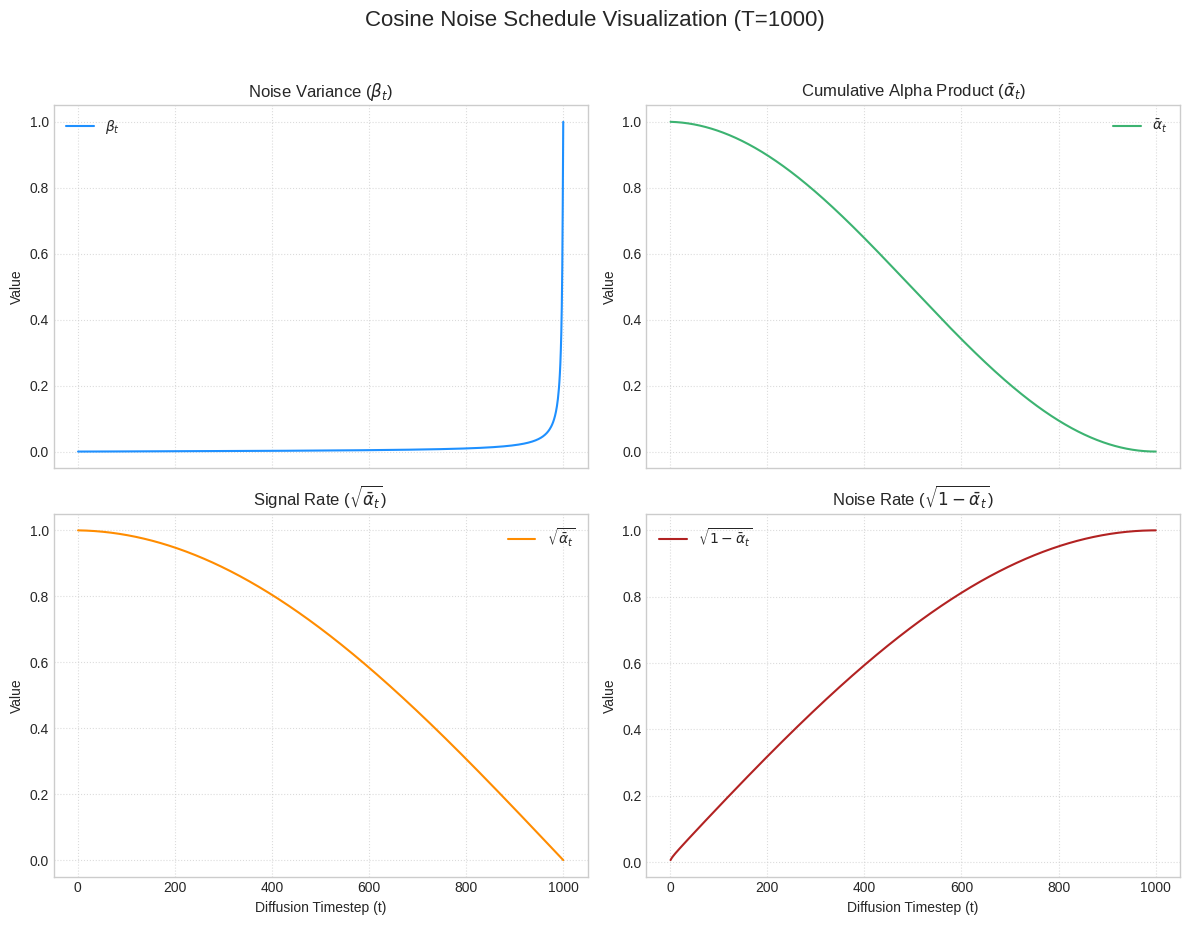
\includegraphics[width=\linewidth]{cosine.png}
          \caption{Visualization of cosine noise schedule}

      \end{figure}

      \text{Time Indexing:}
      \begin{lstlisting}[language=Python,
                            basicstyle=\ttfamily\tiny,
                            numbers=none,
                            frame=single]
index = (t * (n_steps - 1))
    .long()
    .clamp(0, n_steps - 1)
      \end{lstlisting}
    \end{column}
  \end{columns}
\end{frame}

\begin{frame}[fragile]{Forward Process: SDE Implementation}
  \begin{columns}[T]
    \begin{column}{0.5\textwidth}
      \textbf{Forward Process Functions:}
      \begin{lstlisting}[language=Python,
                            basicstyle=\ttfamily\tiny,
                            numbers=none,
                            frame=single]
def marginal_prob(self, x0, t):
    """Get mean & std of q(x_t|x_0)"""
    alpha_t = self.alpha(t).view(-1, 1, 1, 1)
    sigma_t = self.sigma(t)

    mean = alpha_t * x0
    std = sigma_t

    return mean, std

def forward(self, x0, t):
    """Add noise to data: sample from q(x_t|x_0)"""
    mean, std = self.marginal_prob(x0, t)

    z = torch.randn_like(x0)

    x_t = mean + std.view(-1, 1, 1, 1) * z

    return x_t, z
      \end{lstlisting}
    \end{column}

    \begin{column}{0.5\textwidth}
      \textbf{Key Operations:}
      \begin{itemize}\itemsep -0.1cm
        \item \textbf{Get parameters:} $\sqrt{\bar{\alpha}_t}$ and $\sqrt{1-\bar{\alpha}_t}$
        \item \textbf{Calculate mean:} $\mu_t = \alpha_t \cdot \mathbf{x}_0$
        \item \textbf{Sample noise:} $\mathbf{z} \sim \mathcal{N}(\mathbf{0}, \mathbf{I})$
        \item \textbf{Compute noisy image:} $\mathbf{x}_t = \mu_t + \sigma_t \cdot \mathbf{z}$
      \end{itemize}

      \vspace{0.3cm}
      \begin{alertblock}{Implementation Notes}
        \begin{itemize}\itemsep -0.1cm
          \item Forward process enables direct sampling at any timestep $t$
          \item Variance parameters are pre-computed for efficiency
          \item Function returns both $\mathbf{x}_t$ and the noise $\mathbf{z}$ (for training)
          \item Shape management critical for batched operations
        \end{itemize}
      \end{alertblock}
    \end{column}
  \end{columns}
\end{frame}

\begin{frame}{Forward Process Visualization}
  \centering
  \animategraphics[
    controls,
    loop,
    autoplay,
    width=0.9\textwidth
  ]{10}{forward_process/frame_}{001}{074}
  \begin{alertblock}{Forward Process: Clean Image → Pure Noise}
    \begin{itemize}\itemsep -0.1cm
      \item Shows gradual transformation from clean CT image to pure Gaussian noise
      \item Controlled by noise schedule $\beta(t)$ as $t$ increases from 0 to 1
      \item Training objective: Learn to reverse this process by predicting noise $\mathbf{z}$
    \end{itemize}
  \end{alertblock}
\end{frame}

\begin{frame}{cont.}
  \centering
  \begin{figure}
      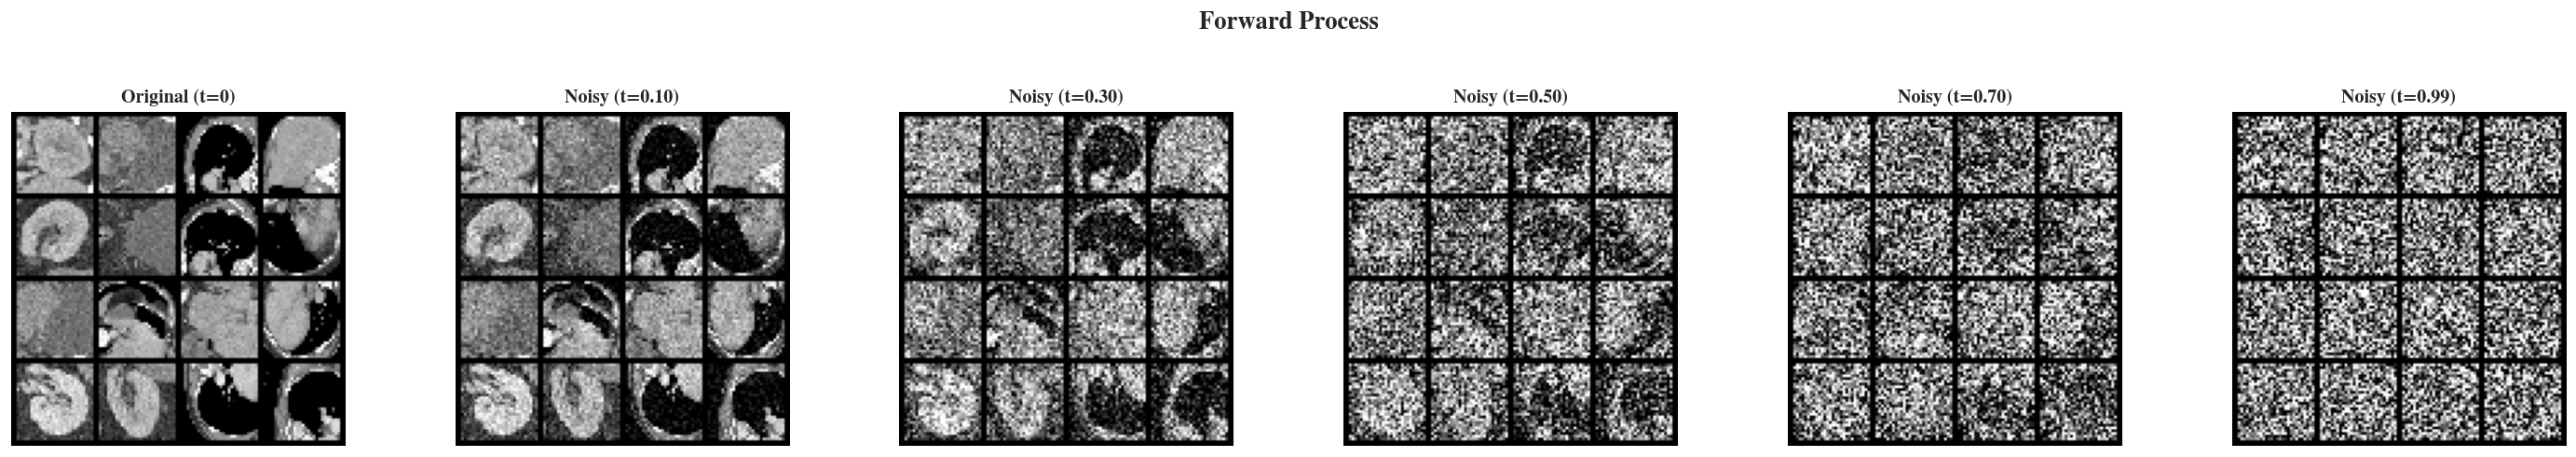
\includegraphics[width=\linewidth]{forward_pass.png}
      \caption{Forward Process}
  \end{figure}
\end{frame}

\section{Model Architecture}

\begin{frame}{Architecture Overview}
  \begin{columns}[T]
    \begin{column}{0.55\textwidth}
        \begin{figure}
            \centering
            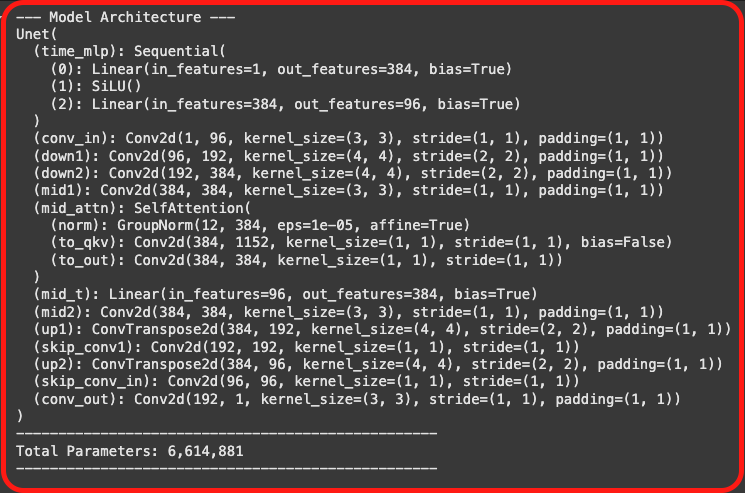
\includegraphics[width=\linewidth]{big_model_arch.png}
            \caption{U‑Net with attention}

        \end{figure}
      \centering
    \end{column}
    \begin{column}{0.45\textwidth}

      \begin{itemize}\itemsep0.2em
        \item \textbf{Input:} Noisy image $\mathbf{x}_t$ \& timestep $t$
        \item \textbf{Encoder:} 3 levels (96 → 192 → 384 channels)
        \item \textbf{Bottleneck:} Self‑attention + time injection
        \item \textbf{Decoder:} Upsample + skip‑connections
        \item \textbf{Output:} Predicted noise $\mathbf{z}$ (same size)
      \end{itemize}
      \vspace{0.5em}
      \textbf{Stats:} 6.6 M parameters, for 28×28 CT patches
    \end{column}
  \end{columns}
\end{frame}

\begin{frame}[fragile]{Time Conditioning \& Self‑Attention}
  \begin{columns}[T]
    \begin{column}{0.48\textwidth}
      \textbf{Time Conditioning:}\\
      Embed continuous timestep \(t\) into a feature vector and inject at the bottleneck.
      \medskip
      \scriptsize
      \begin{lstlisting}[language=Python,
                            basicstyle=\ttfamily\tiny,
                            numbers=none,
                            frame=single]
self.time_mlp = nn.Sequential(
  nn.Linear(1, hidden_dim*4),
  nn.SiLU(),
  nn.Linear(hidden_dim*4, hidden_dim)
)

h += self.mid_t(t_emb).view(-1, hidden_dim, 1, 1)
      \end{lstlisting}
      \normalsize
    \end{column}

    \begin{column}{0.52\textwidth}
      \textbf{Self‑Attention Block :}\\
      Multi‑head attention lets each pixel gather context from all others.
      \medskip
      \scriptsize
      \begin{lstlisting}[language=Python,
                            basicstyle=\ttfamily\tiny,
                            numbers=none,
                            frame=single]
class SelfAttention(nn.Module):
    def __init__(self, channels, num_heads=8):
        self.scale = (channels//num_heads)**-0.5
        self.to_qkv = nn.Conv2d(channels, channels*3, 1, bias=False)
        self.to_out = nn.Conv2d(channels, channels, 1)

    def forward(self, x):
        B,C,H,W = x.shape
        qkv = self.to_qkv(x).chunk(3, dim=1)
        q,k,v = [t.view(B, -1, H*W)
                   .reshape(B, h, d, H*W)
                   .permute(0,1,3,2)
                 for t,(h,d) in zip(qkv, [(8,C//8)]*3)]
        attn = torch.softmax((q @ k.transpose(-1,-2))*self.scale, -1)
        out = (attn @ v).permute(0,1,3,2).reshape(B,C,H,W)
        return self.to_out(out) + x
      \end{lstlisting}
      \normalsize
    \end{column}
  \end{columns}
\end{frame}

\section{Training}

\begin{frame}{Loss Function}
  \begin{columns}[T]
    \begin{column}{0.55\textwidth}
      \textbf{1. Noise Prediction Loss (MSE):}
      \vspace{0.3em}
      \[
        \mathcal{L}_{\mathrm{noise}}
        = \mathbb{E}\Bigl[\|\mathbf{s}_\theta(\mathbf{x}_t,t) - \mathbf{z}\|^2\Bigr]
      \]

      \vspace{0.5em}
      \textbf{2. Frequency‑Domain Loss (L1):}
      \vspace{0.3em}
      \[
        \mathcal{L}_{\mathrm{freq}}
        = \mathbb{E}\Bigl[\|\;|\mathcal{F}(\hat{\mathbf{x}}_0)| - |\mathcal{F}(\mathbf{x}_0)|\|_1\Bigr]
      \]
      \small\emph{\(\mathcal{F}\)=2D FFT, \(|\cdot|\)=magnitude}\normalsize

      \vspace{0.5em}
      \textbf{3. Combined Objective:}
      \vspace{0.3em}
      \[
        \mathcal{L}_{\mathrm{total}}
        = \mathcal{L}_{\mathrm{noise}}
        + \lambda\,\mathcal{L}_{\mathrm{freq}}
        \quad(\lambda=0.1)
      \]

      \vspace{0.8em}
      \scriptsize
      \textit{%
        $\mathbf{x}_t$: noisy image at time $t$; \quad
        $\mathbf{x}_0$: ground‑truth clean image; \quad
        $\hat{\mathbf{x}}_0$: reconstructed image; \quad
        $\mathbf{z}$: sampled Gaussian noise; \quad
        $\mathbf{s}_\theta(\cdot)$: score network (predicted noise); \quad
        $\lambda$: frequency‐loss weight
      }
    \end{column}

    \begin{column}{0.45\textwidth}
      \centering
        \begin{figure}
            \centering
            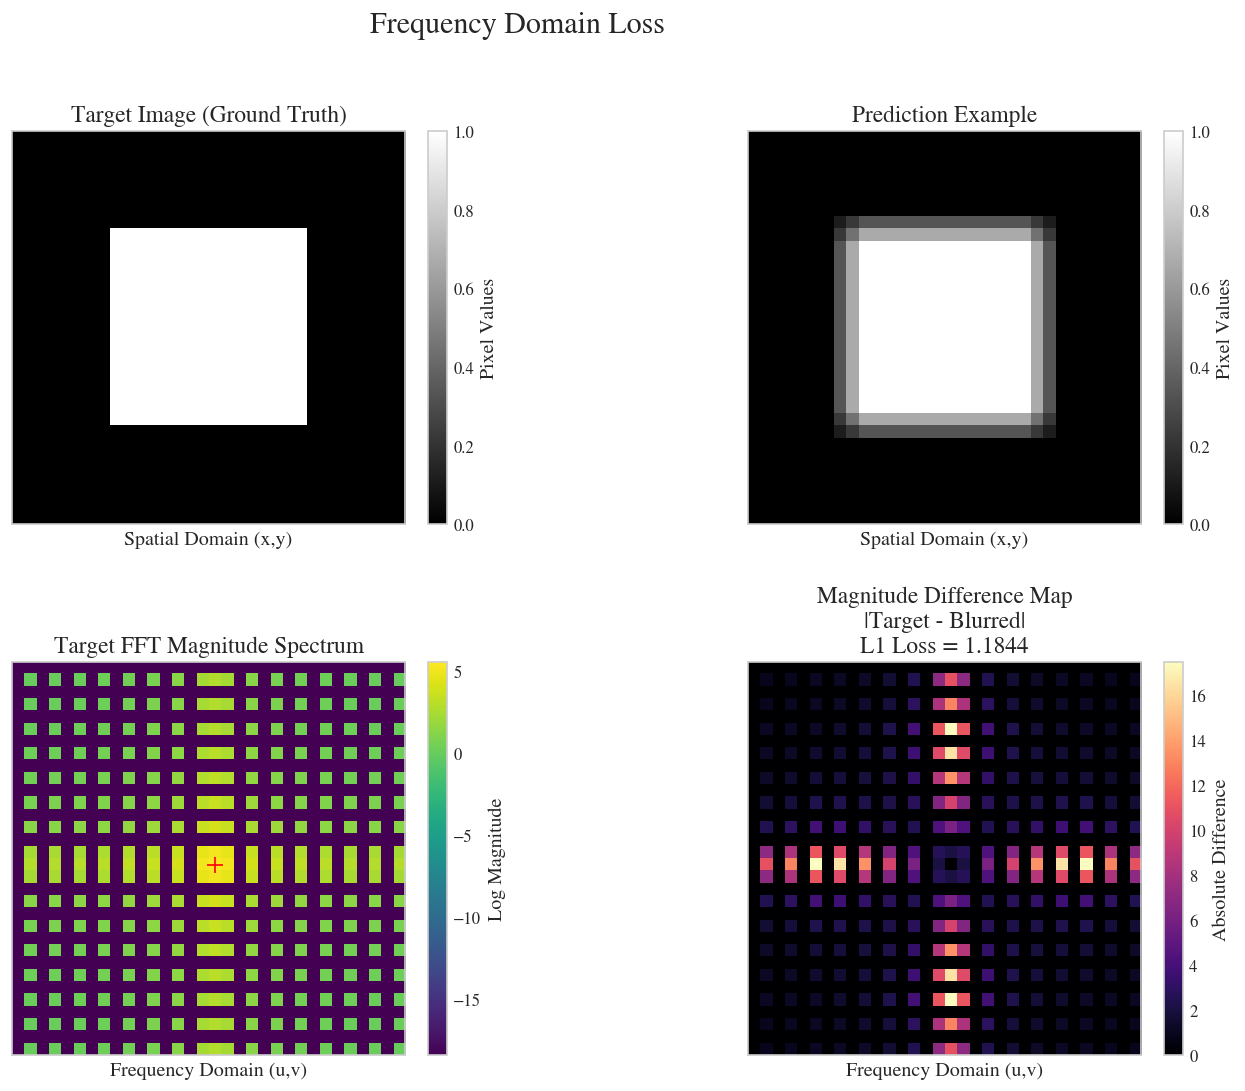
\includegraphics[width=\linewidth]{freq_domian_loss.png}
            \caption{FFT Domain Loss example}

        \end{figure}
    \end{column}
  \end{columns}
\end{frame}

\begin{frame}[fragile]{Implementation of Loss Components}

  \begin{columns}[T]

    \begin{column}{0.5\textwidth}
      \begin{lstlisting}[language=Python,
                            basicstyle=\ttfamily\tiny,
                            numbers=none,
                            frame=single]
def diffusion_loss(model, sde, x0, lambda_freq=0.1):
{
    t = torch.rand(x0.size(0), device=x0.device)
    x_t, z = sde.forward(x0, t)

    z_pred = model(x_t, t)
    loss_noise = F.mse_loss(z_pred, z)

    alpha = sde.alpha(t).view(-1,1,1,1)
    sigma = sde.sigma(t).view(-1,1,1,1)
    x0_pred = (x_t - sigma*z_pred) / alpha
    loss_freq = frequency_domain_loss(x0_pred, x0)

    total = loss_noise + lambda_freq * loss_freq
    return total, loss_noise, loss_freq
}
      \end{lstlisting}
    \end{column}

    \begin{column}{0.5\textwidth}
       \begin{lstlisting}[language=Python,
                            basicstyle=\ttfamily\tiny,
                            numbers=none,
                            frame=single]
def frequency_domain_loss(pred_x0, target_x0, norm='l1'):
{
    pred_x0 = pred_x0.float()
    target_x0 = target_x0.float()

    pred_fft = torch.fft.fft2(pred_x0, dim=(-2,-1))
    target_fft = torch.fft.fft2(target_x0, dim=(-2,-1))

    pred_mag = torch.abs(pred_fft)
    target_mag = torch.abs(target_fft)

    loss = F.l1_loss(pred_mag, target_mag)
    return loss
}
      \end{lstlisting}
    \end{column}

  \end{columns}

  \vspace{-0.3cm}
  \begin{alertblock}{Why add a frequency loss?}
    \footnotesize
    \begin{itemize} \itemsep 0pt
      \item Aims to preserve high‑frequency details often lost with pure MSE.
      \item Aligns spectral content between prediction \& target images.
      \item Can potentially improve perceptual quality and structure preservation.
    \end{itemize}
  \end{alertblock}

\end{frame}

\begin{frame}{Optimization \& Training Progress}
  \begin{columns}[T]
    \begin{column}{0.45\textwidth}
      \textbf{Optimizer \& Hyperparameters}
      \begin{itemize}\small\itemsep0.2em
        \item \textbf{Optimizer:} AdamW (wd=1e-4)
        \item \textbf{LR:} 5e-5 w/ CosineAnnealingWarmRestarts
        \item \textbf{Batch size:} 64
        \item \textbf{Epochs:} 100
        \item \textbf{Loss Fn:} MSE($\mathbf{z}_\text{pred}, \mathbf{z}$) + 0.1 $\times$ L1(FFT Mag)
        \item \textbf{Grad clip:} max‐norm 1.0
      \end{itemize}

      \medskip
      \textbf{Final Loss Values (Epoch 100):}
      \begin{itemize}\small\itemsep0.2em
        \item \textbf{Train Total:} 0.51
        \item \textbf{Validation Total:} 0.77
      \end{itemize}

    \end{column}
    \begin{column}{0.55\textwidth}
      \centering
      \begin{figure}
        \centering
        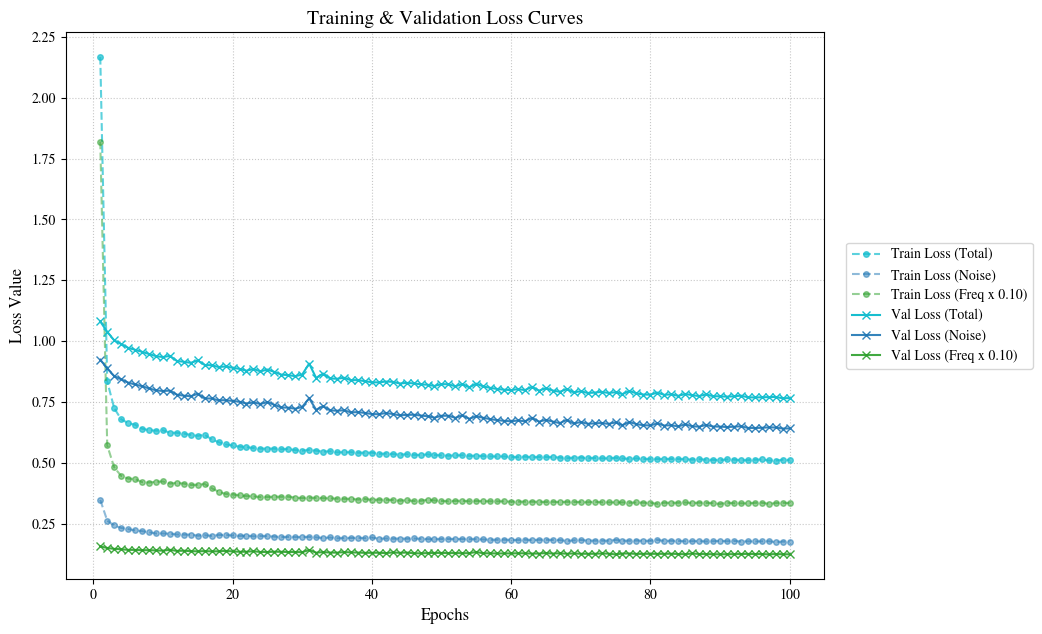
\includegraphics[width=\linewidth]{loss_curve.png}
        \caption{Training \& validation loss (Total) over epochs.}
      \end{figure}
    \end{column}
  \end{columns}
\end{frame}

\section{Inference}

\begin{frame}[fragile]{Generative Denoising Algorithm}
  \begin{columns}[T]
    \begin{column}{0.55\textwidth}
      \small
      \begin{lstlisting}[language=Python,
                            basicstyle=\ttfamily\tiny,
                            numbers=none,
                            frame=single]
@torch.no_grad()
def generative_denoising(y_noisy, model, sde,
                          sigma_n, n_steps, eps=1e-5):
    x = torch.randn_like(y_noisy)
    time_steps = torch.linspace(1.0, eps, n_steps+1)

    for i in range(n_steps):
        t_curr, t_next = time_steps[i], time_steps[i+1]
        t_vec = torch.full((x.size(0),), t_curr, device=x.device)

        σ_t = sde.sigma(t_vec).view(-1,1,1,1)
        λ_t = σ_t**2 / (σ_t**2 + sigma_n**2)
        x = (1-λ_t)*x + λ_t*y_noisy

        z_pred = model(x, t_vec)
        α_t = sde.alpha(t_vec).view(-1,1,1,1)
        x0_pred = (x - σ_t*z_pred) / α_t
        x0_pred.clamp_(-1,1)

        mean, std = sde.marginal_prob(x0_pred, t_next)
        z = torch.randn_like(x) if i < n_steps-1 else 0
        x = mean + std.view(-1,1,1,1)*z

    return x0_pred
      \end{lstlisting}
    \end{column}

    \begin{column}{0.45\textwidth}
      \textbf{Key Steps:}
        \begin{itemize}\small\itemsep0.5em
    \item \textbf{Initialization:}
      $\displaystyle x_T\sim\mathcal{N}(0,I)$ as starting noise.
    \item \textbf{Measurement Conditioning:}
      $\lambda_t=\frac{\sigma_t^2}{\sigma_t^2+\sigma_n^2}$,
      then $x_t\leftarrow(1-\lambda_t)x_t+\lambda_t\,y$.
    \item \textbf{Score Estimation:}
      Predict noise with $\mathbf{s}_\theta(x_t,t)=z_\text{pred}$.
    \item \textbf{Clean Estimate (Tweedie):}
      $\hat x_0=(x_t-\sigma_t\,z_\text{pred})/\alpha_t$.
    \item \textbf{Reverse SDE Sampling:}
      Draw $x_{t-\Delta t}\sim\mathcal{N}(\mu,\sigma^2)$ from the learned posterior.
    \end{itemize}
    \end{column}
  \end{columns}
\end{frame}

\begin{frame}{Reverse Process Visualization}
  \centering
  \animategraphics[
    controls,
    loop,
    autoplay,
    width=0.4\textwidth
  ]{10}{reverse_process/frame_}{001}{050}

  \begin{alertblock}{Reverse Process: Noise → Clean Image}
    \begin{itemize}\itemsep -0.1cm
      \item Shows the generative denoising process from random noise to clean reconstruction
      \item Algorithm iteratively refines estimate while maintaining consistency with noisy input
      \item Uses 1000 denoising steps to balance detail recovery and stability
    \end{itemize}
  \end{alertblock}
\end{frame}

\begin{frame}{cont.}
  \centering
  \begin{figure}
      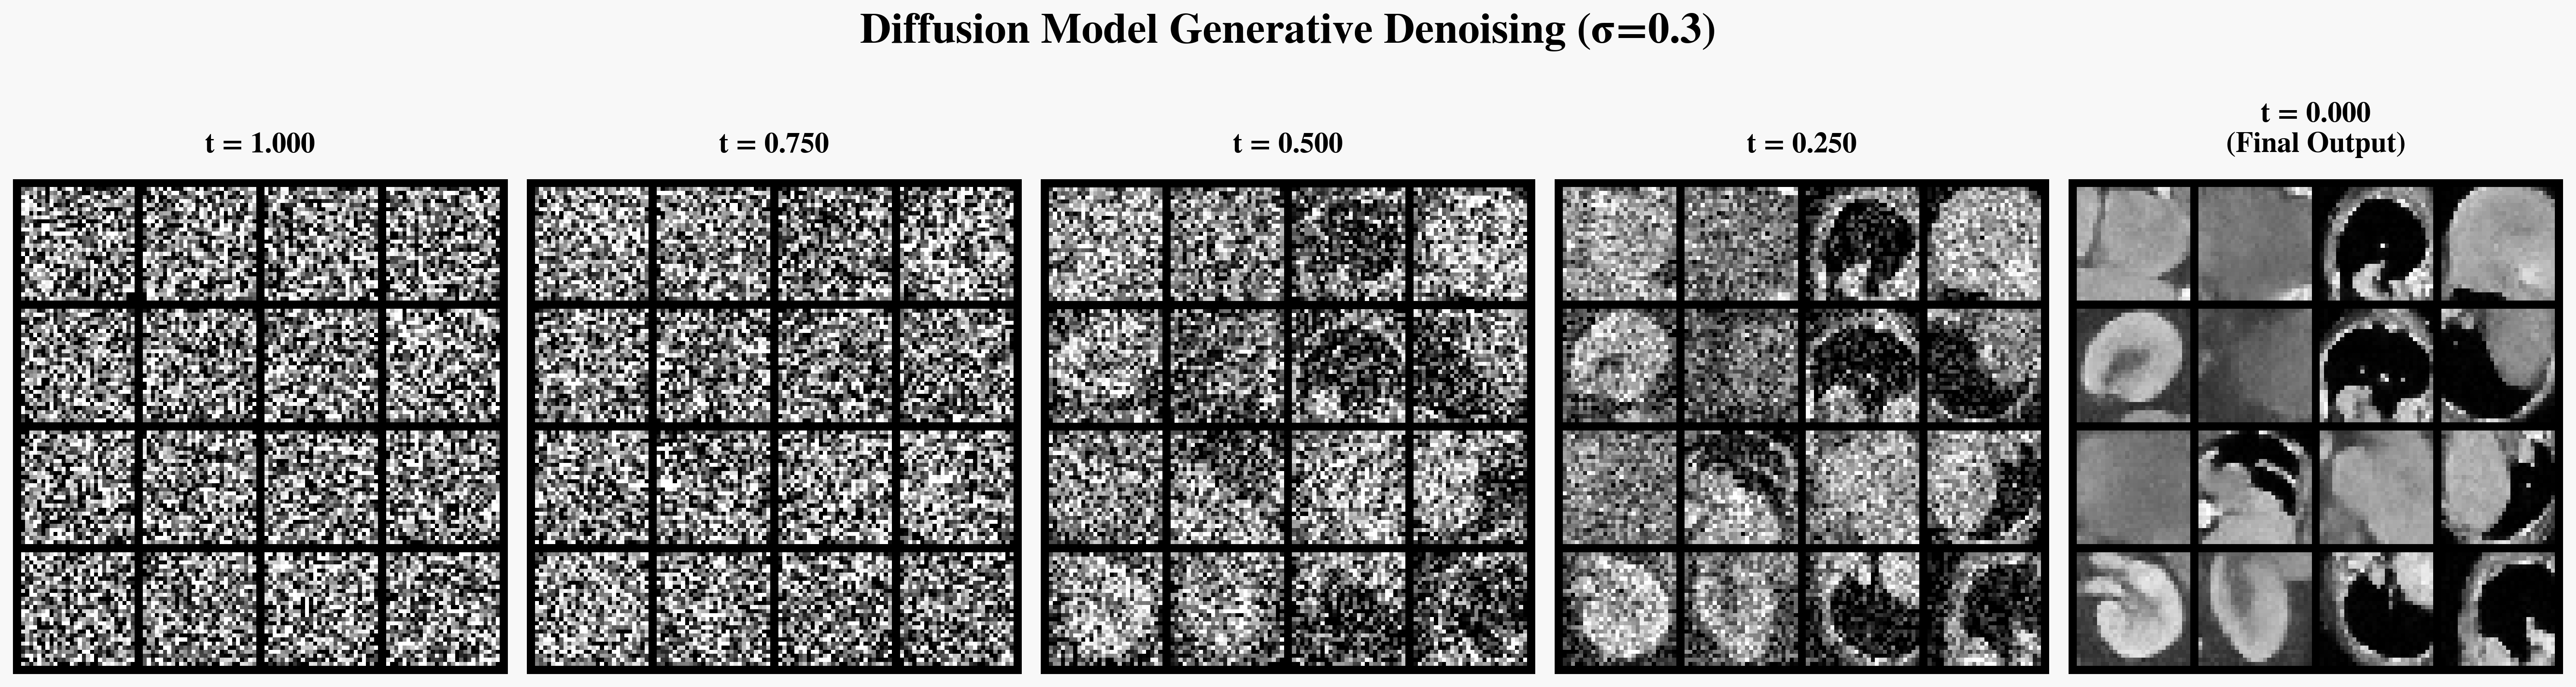
\includegraphics[width=\linewidth]{reverse_process_snapshots.png}
      \caption{Reverse Process}
  \end{figure}
\end{frame}

\section{Results}

\begin{frame}{Results}

  \begin{figure}
    \centering

    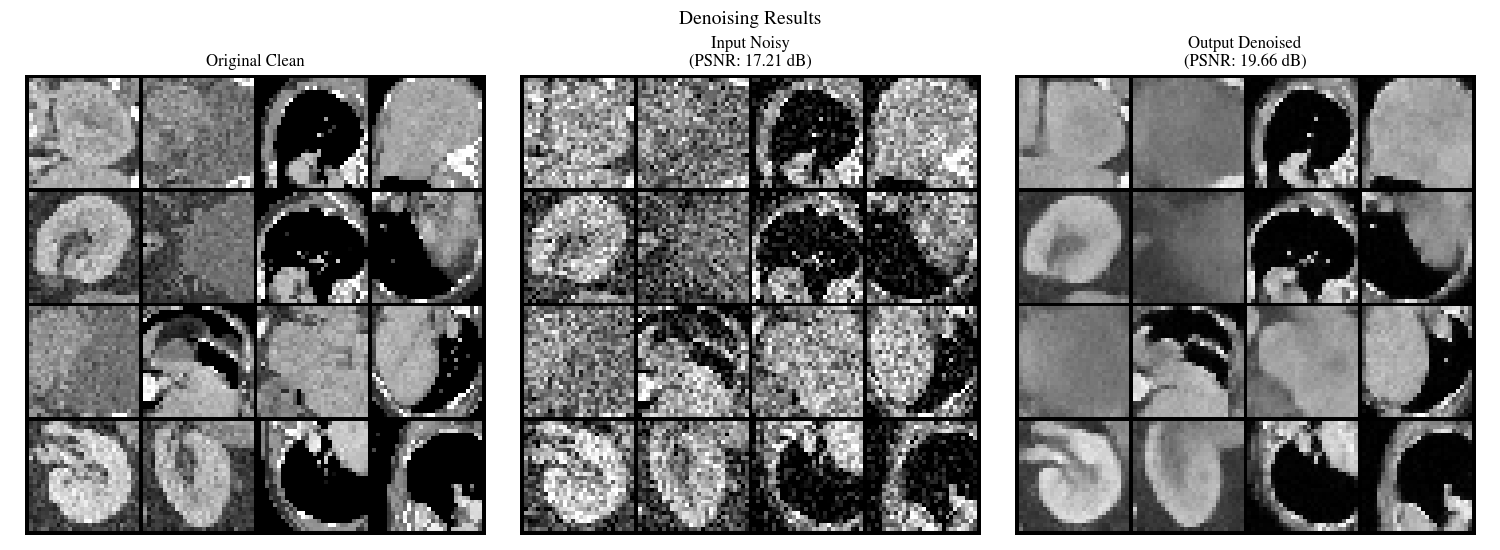
\includegraphics[width=0.9\textwidth]{final_comparison.png}

    \caption{\footnotesize Comparison: Ground Truth (left), Noisy Input ($\sigma_n=0.3$, middle), Denoised Output (right)}
  \end{figure}

  \vspace{-0.2cm}

  \begin{block}{Evaluation Setup}
    \footnotesize
    \begin{itemize} \itemsep 0pt
        \item \textbf{Test Data:} 16 OrganAMNIST patches (unseen during training).
        \item \textbf{Input Noise:} Additive White Gaussian Noise (AWGN) with $\sigma_n = 0.3$.
        \item \textbf{Denoising:} $N=1000$ reverse diffusion steps.
    \end{itemize}
  \end{block}

\end{frame}

\begin{frame}{Quantitative Results \& Key Findings}
  \textbf{Quantitative Metrics}
  \begin{table}
    \centering
    \small
    \begin{tabular}{lcc}
      \toprule
      Image           & PSNR (dB) ↑ & SSIM ↑ \\
      \midrule
      Noisy Input     & 17.21       & 0.5372 \\
      Denoised Output & 19.66       & 0.5364 \\
      \midrule
      \textbf{Improvement} & \textbf{+2.44} & \textbf{–0.0008} \\
      \bottomrule
    \end{tabular}
  \end{table}
  \vspace{0.5em}
\begin{alertblock}{Key Findings}
  \begin{itemize}\small\itemsep0.3em
    \item \textbf{+2.44 dB PSNR gain} demonstrates the model how to effectively remove Gaussian noise.
    \item \textbf Anatomical details preserved despite minor SSIM change.
    \item \textbf{Fine-detail recovery} (e.g.\ vessel edges, tissue boundaries) is improved by the frequency-domain loss term.
    \item \textbf{Conditional generative denoising} yields diverse, realistic reconstructions based on provided noisy input
  \end{itemize}
\end{alertblock}

\end{frame}

\section{Conclusions \& Future Work}
\begin{frame}{Conclusions \& Future Work}
  \begin{columns}[T]
    \begin{column}{0.45\textwidth}
      \textbf{Conclusions}
      \begin{itemize}\small\itemsep 0.2em
        \item Successfully applied conditional diffusion for denoising medical patches.
        \item Achieved significant PSNR gain (+2.44 dB); details preserved visually.
        \item Demonstrated potential for generative models in low-data medical imaging.
      \end{itemize}
      \vfill
    \end{column}

    \begin{column}{0.55\textwidth}
      \textbf{Future Work}
      \footnotesize
      \begin{itemize}\itemsep -0.1em
        \item \textbf{Physics-Informed:} Incorporate forward model ($\op{A}$) for inverse problems \cite{song2022solvinginverseproblemsmedical}; explore diffusion directly on measurement data (e.g., sinograms) \cite{song2021scorebasedgenerativemodelingstochastic}.

        \item \textbf{Scale \& Efficiency:} Extend models to full 2D slices / 3D volumes; investigate faster sampling (e.g., ODE solvers).

        \item \textbf{Hybrid Methods:} Combine generative prior with classical data-fidelity terms (inspired by ML/MAP \cite{4307558}).

        \item \textbf{Clinical Validation:} Evaluate on realistic phantom/patient data; compare with clinical benchmarks \& MGH prototypes.
      \end{itemize}
    \end{column}
  \end{columns}
\end{frame}
\begin{frame}[allowframebreaks]{References}

    \printbibliography

\end{frame}

\begin{frame}{Thank You \& Questions}
  \centering
  {\Large Thank you! \\[1em]
  I’m happy to take any questions!}
\end{frame}


\end{document}
